\chapter{DreamDateのプロトタイピングと機能}
\label{chap:search}


この章ではではDreamDateがスマートフォンアプリで睡眠中に音を流すという形に至った背景を述べる。

\section{刺激提示のプロトタイピング}
 人には視覚、聴覚、触覚、味覚、嗅覚を含む5つの感覚器がある。本研究ではそのうちの聴覚と嗅覚による刺激が睡眠中の夢に与える影響を実験を通して観察した。

\subsection{香りによる刺激}
\begin{figure}[htbp]
\begin{center}
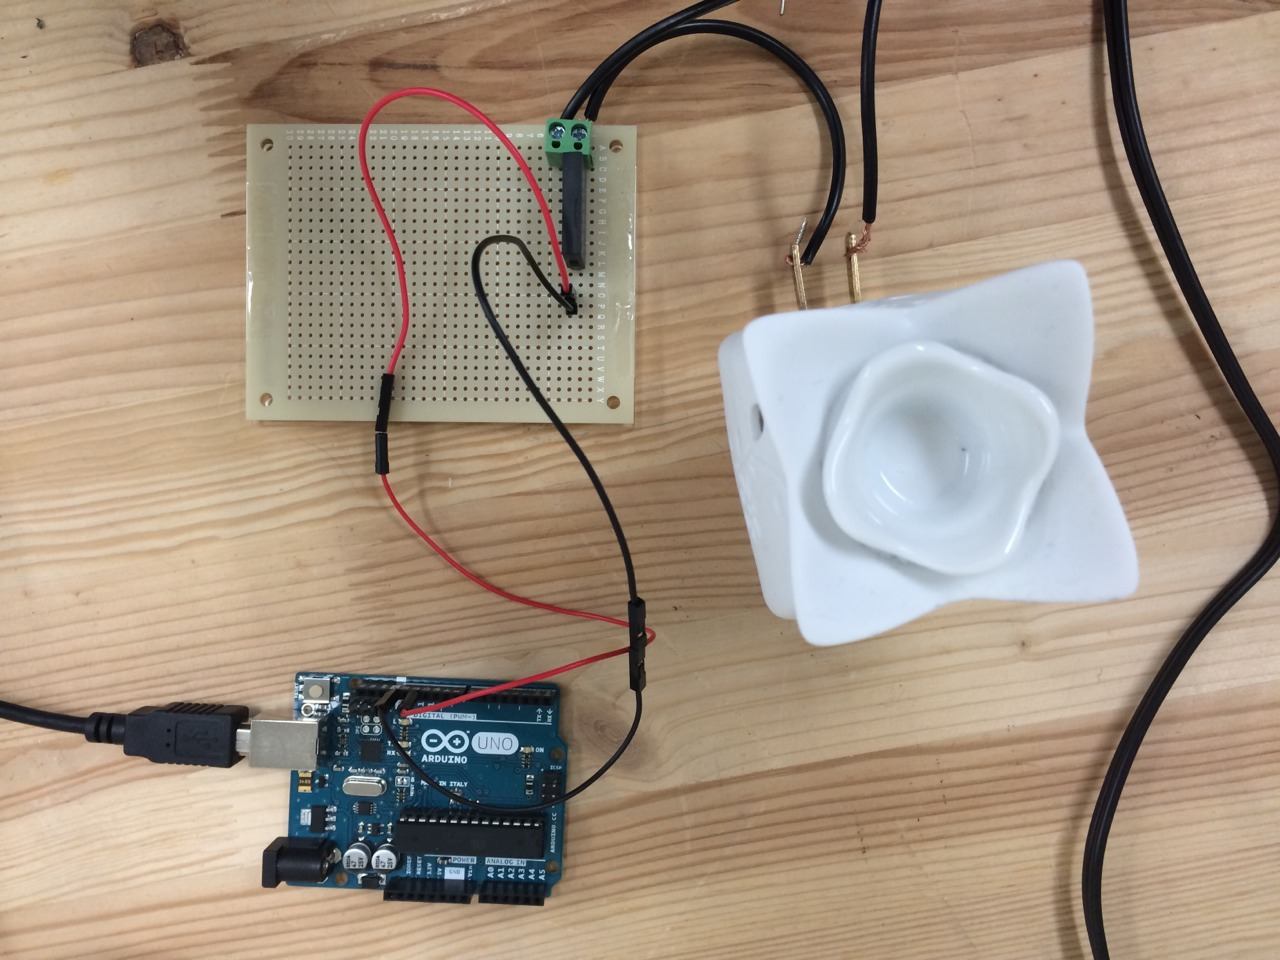
\includegraphics[width=9cm]{eps/smell.eps}
\caption{香りによる刺激}
\label{smell}
\end{center}
\end{figure}

 ラベンダーやバラのような良い香りは睡眠に良い影響を与え、心地良い夢を見やすくするということはMichael SchredlとBoris Stuckの研究によって証明されている\cite{roseDream}。しかし香りが夢の内容に影響を与えるか否かの研究はまだ行われていない。そこでこのプロトタイプはREM睡眠の時に思い出と直結する香りを出して夢を刺激することで夢になんらかの影響を与えられるものか否かを確かめるために製作した。\\
 加速度センサーでREM睡眠を検出したらアロマランプに光がつき、5分後香りが部屋中に充満するという作りになっている。図\ref{smell}にあるのはそのプロトタイプの写真だ。\\
 実験に参加したのは嗅覚が正常に機能している(風邪などを引いていない)22歳の女性3名だ。被験者1には交際相手が部屋で使っているアロマとコーヒー豆の香りで刺激した。被験者2と被験者3はコーヒー豆の香りで刺激した。その香りをたくとすぐに過去の思い出と直感的に繋がる香りをあえて選んだ。またアロマライトは被験者の頭のすぐ横に置いた。\\
 2015年の1月に10日間の実験を行った。香りありの夜、香りなしの夜を5日間ずつ交互に繰り返した。その結果が以下の図\ref{smellExperiment}の通りだ。

\subsection{音による刺激}
 同じ被験者に今度は香りではなく音によるインプットをしてもらった。REM睡眠中に海の音や交際相手と一緒に聞いた音楽を流した。すると音によっては起こされてしまったり、被験者によっては全く影響が出ないという結果になった。しかし、図\ref{smellExperiment}が示すように、香りのインプットでは影響が全くなかったのに比べ、音のインプットは被験者1、被験者2ともに音による刺激で1日だけ夢を観たことがわかった。

\begin{figure}[htbp]
\begin{center}
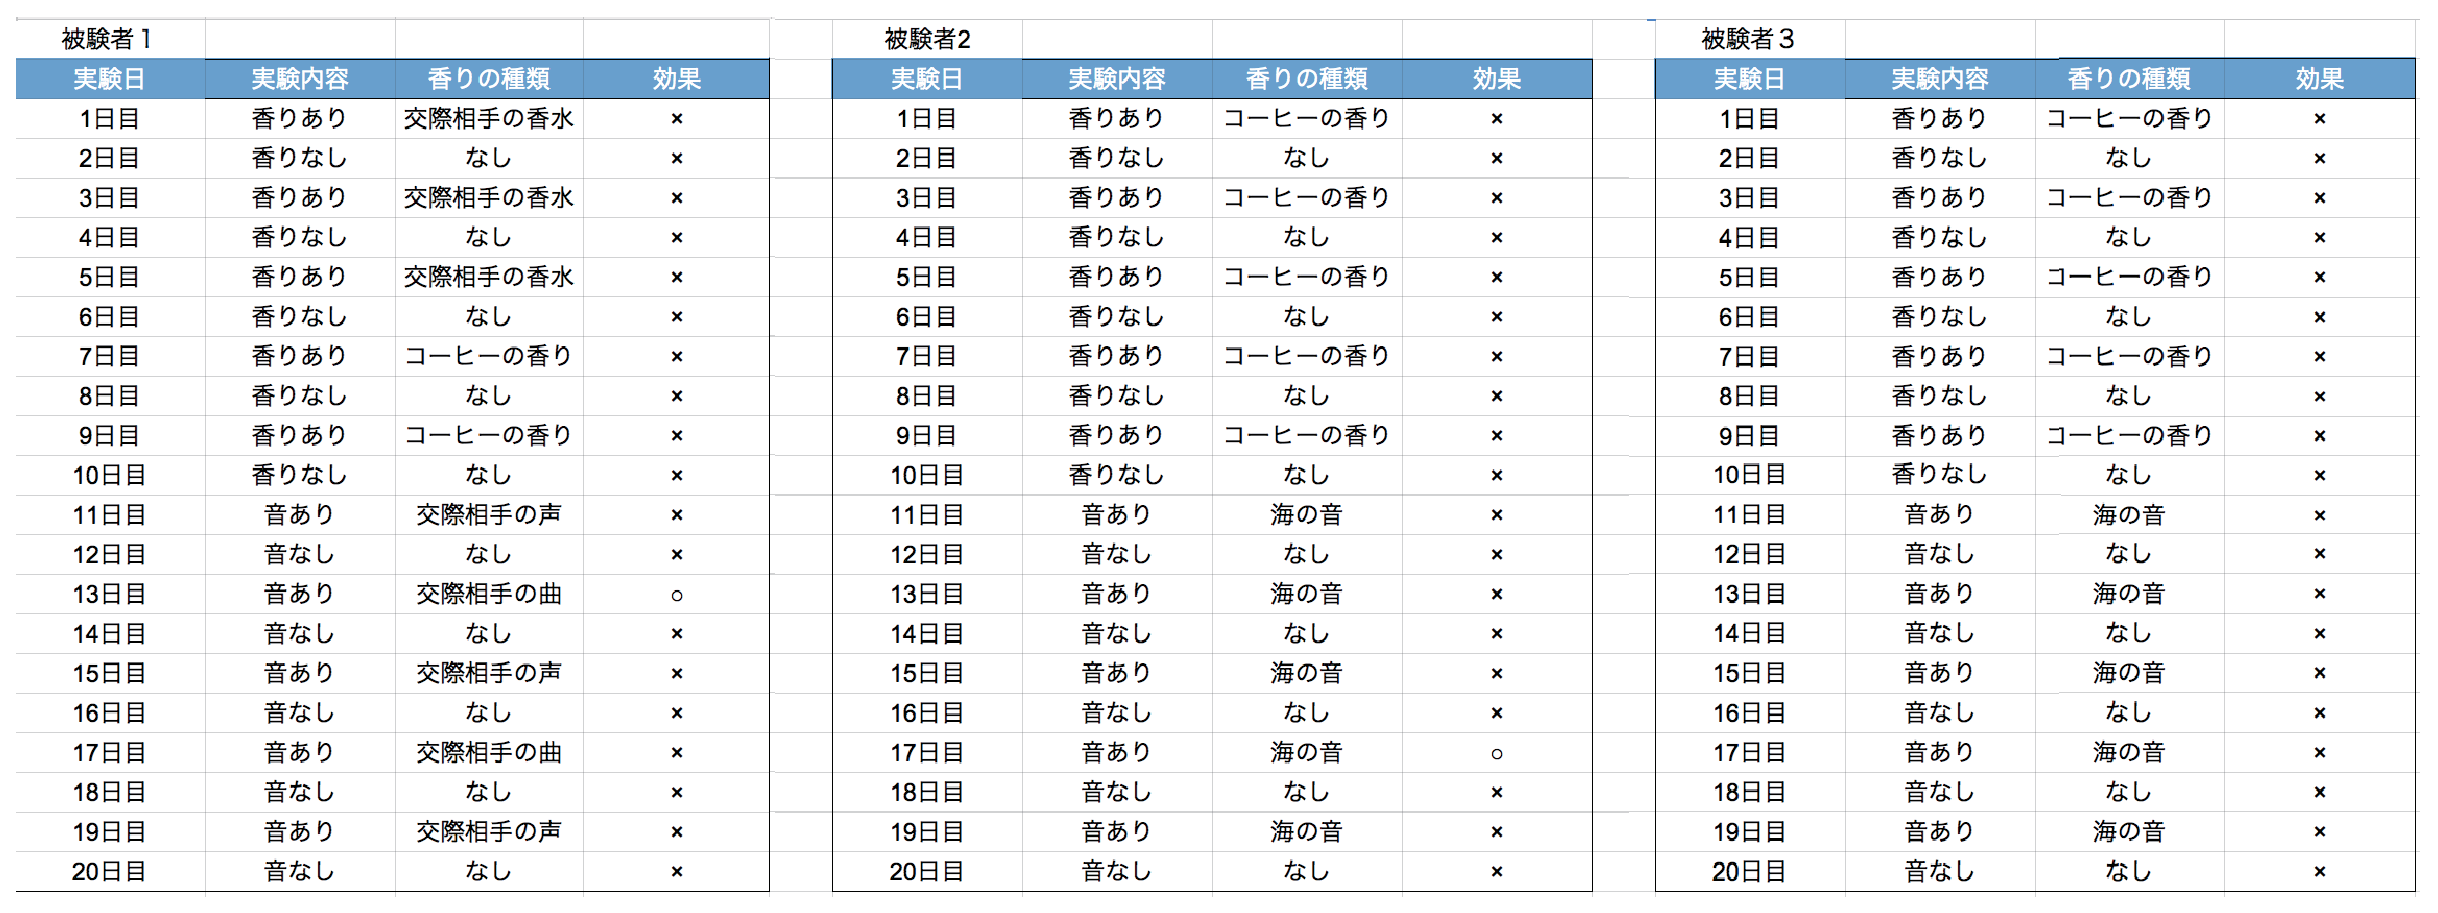
\includegraphics[width=15cm]{eps/smellExperiment.eps}
\caption{香りによる刺激の実験結果}
\label{smellExperiment}
\end{center}
\end{figure}

\section{睡眠観測のプロトタイピング}
ユーザーの睡眠深度のモニタリング方法はいくつかある。それぞれの方法をユーザビリティと機能性の2つの観点から、実験を通して分析する。

\subsection{脳波センサーによる観測}
 このプロトタイプではNeuroSkyのThinkGear ASICモジュールという脳波センサーを使用した。Theta波が4〜7.2HzかつDelta波が0.5〜4Hzである時をREM睡眠中であるとし自らが実験台となり装着して寝てみた。しかしこの手法は頭を締め付けられる感覚があり、且つ汗をかいてしまうのでユーザーに負担がかかる。寝心地を損ねてしまうということがわかりセンサーの体と離す別の方法を試すことにした。
\begin{figure}[htbp]
\begin{center}
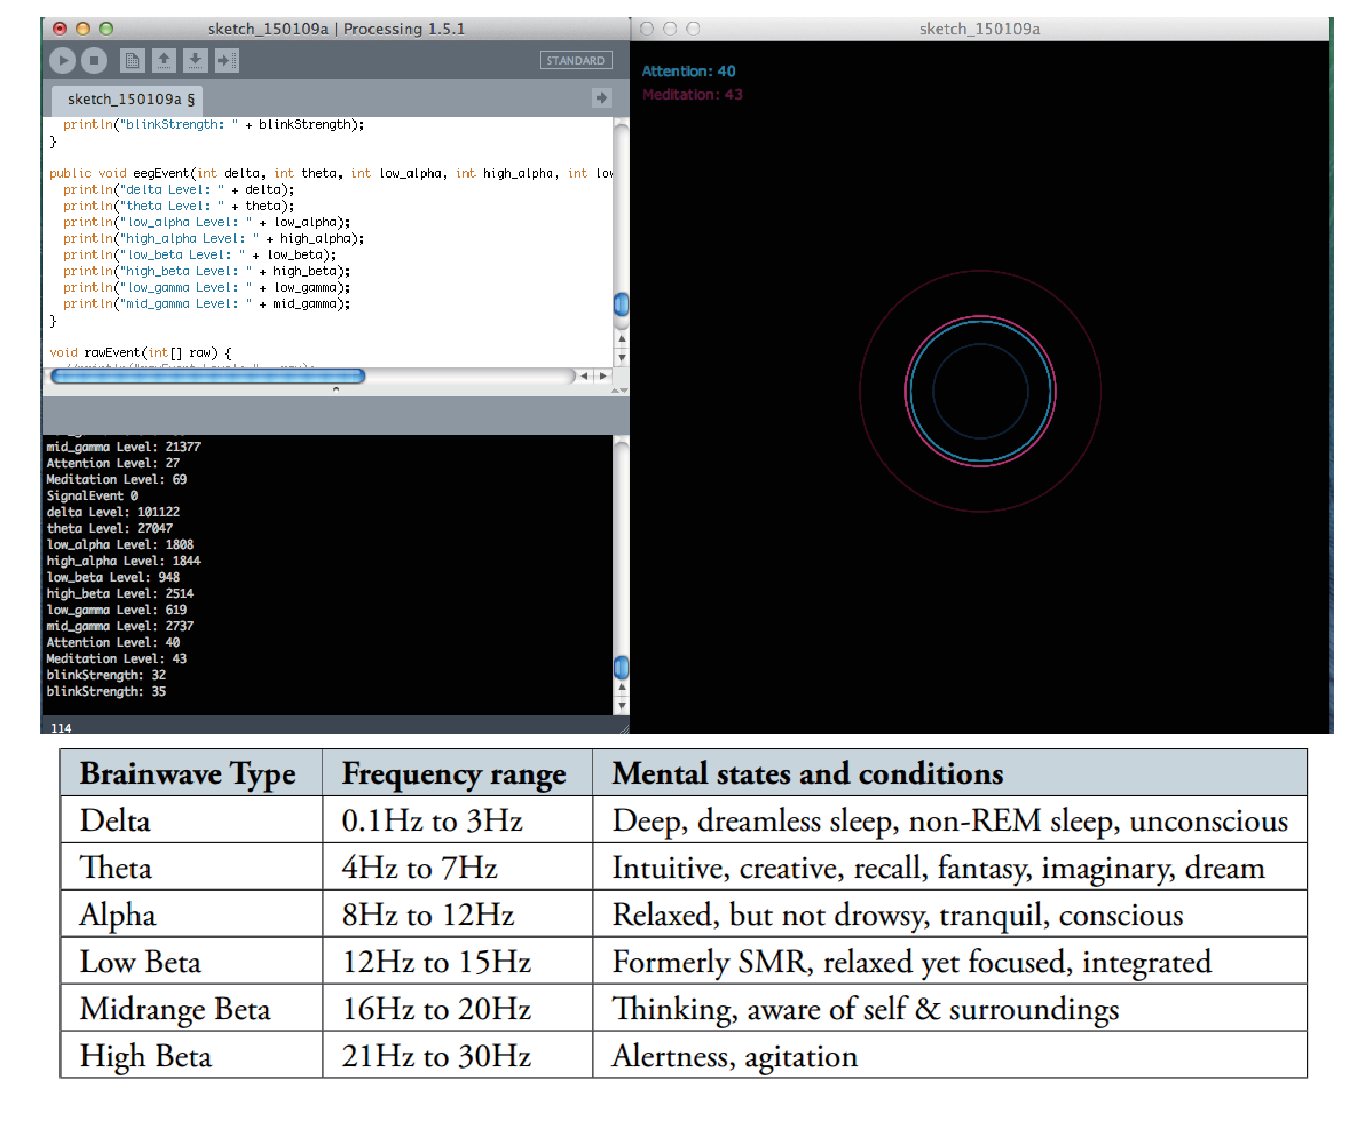
\includegraphics[width=10cm]{eps/brainWave.eps}
\caption{脳波センサーによるセンシングのプログラムと睡眠ステージと脳波の数値}
\label{brainWave}
\end{center}
\end{figure}

\subsection{心拍センサーによる観測}
 次に市販で売られている心拍センサーを追懐睡眠中の心拍数を観測することでREM睡眠を検出できるかどうかの実験をした。しかし寝ているときに指にセンサーを装着するのは発汗のを引き起こし、ユーザー体験の視点から非常に好ましくないということがわかりまたしても別の方法を試すことにした。

\begin{figure}[htbp]
\begin{center}
\includegraphics[width=10cm]{eps/heart.eps}
\caption{心拍センサーによるセンシング}
\label{heart}
\end{center}
\end{figure}

\subsection{kinectによる観測}
 このプロトタイプはKinectを使用して、ユーザーの寝返りを検知して音楽を流すシステムである。図\ref{kinect}のようにkinectを天井に設置する。ウェラブルセンサーではないためユーザには負担がかからない。但し布団をかぶってしまうとkinectによる骨格トラッキングは難しい。そのためOpenCVのライブラリを利用して、画像処理を行った。\\
 寝返り判定の正確性を確かめるために、実際にベッドの上で寝返りを打ったとき音が鳴るかを試したところ、開発したプログラミングではノイズが多く出て誤作動が起きてしまうのでkinectを使うのは適切ではないと判断した。しかしプログラミングの能力が高い人により開発されれば、kinectによるトラッキングの精度もあげられるはずである。ただし、デバイス自体の価格が高いのと、取り付けに労力が必要とされることと、ポータブルではないため旅先では使えないという点で、本研究では好ましくないとした。

\begin{figure}[htbp]
\begin{center}
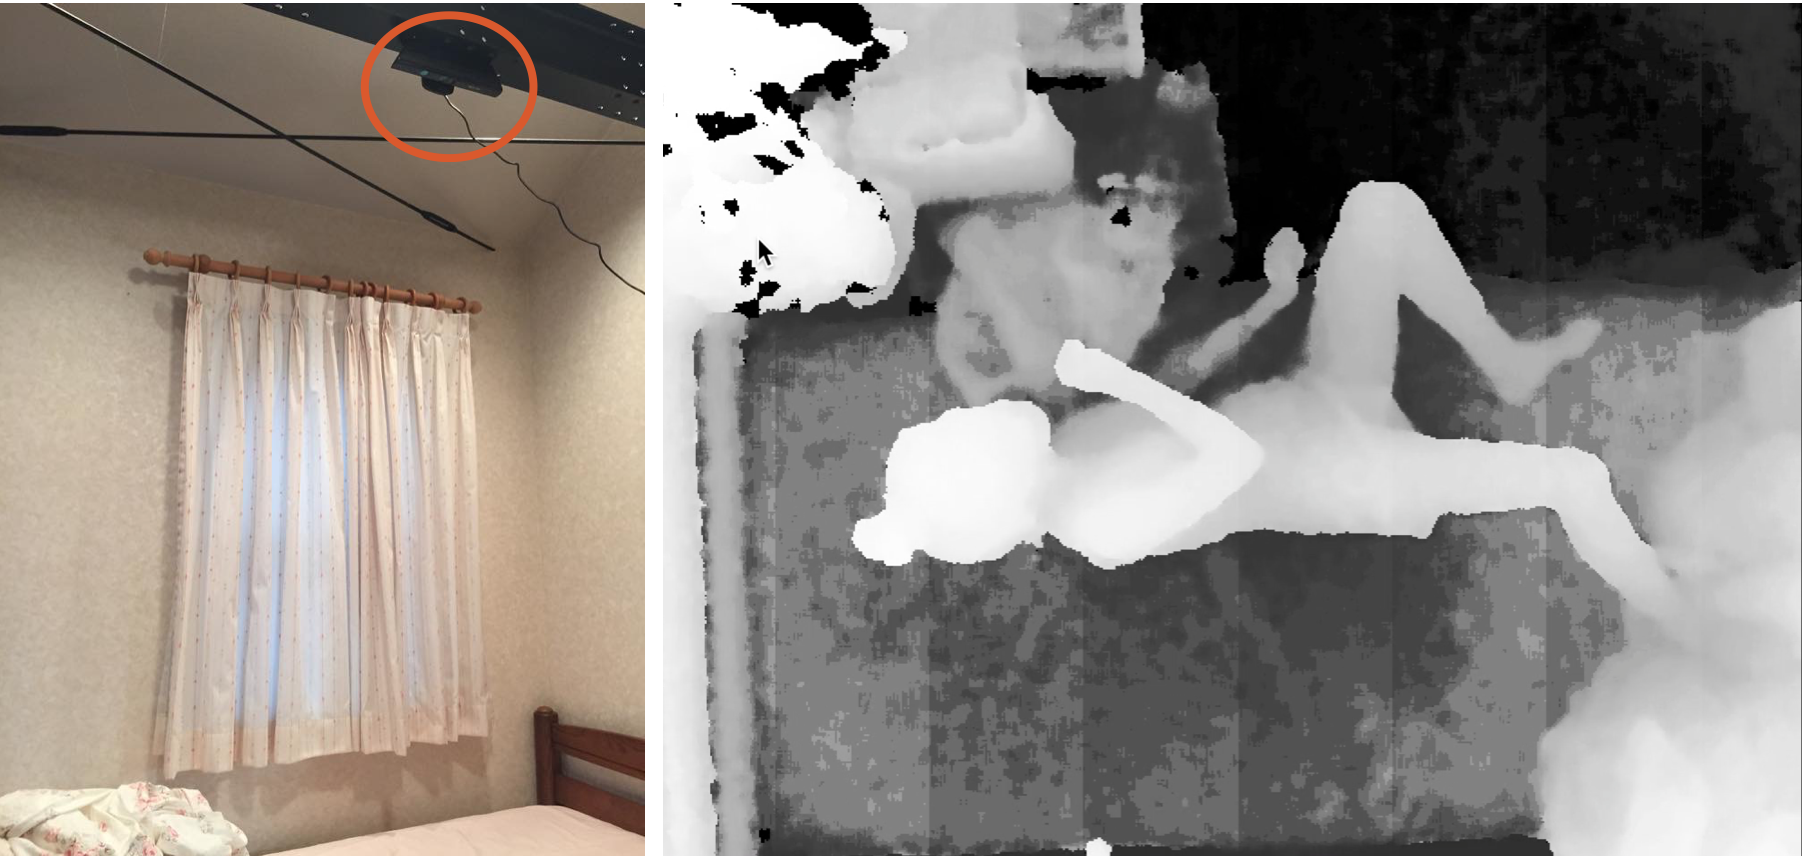
\includegraphics[width=15cm]{eps/kinect.eps}
\caption{kinectによるセンシング}
\label{kinect}
\end{center}
\end{figure}

\subsection{スマートフォンの加速度センサによる観測}
 最終的に多くの人々が既に使用していて、ユーザビリティーの視点から見てもっとも負担のかからないスマートフォンアプリケーションによるセンシングに試みた。スマートフォンで計測すときはウェラブルではないため身軽であるし、持ち運びが簡単なので旅中も使える。スマートフォンアプリケーションによるセンシング方法とその正確性については5章で述べる。

\section{実装}
\subsection{機能}
 現在、仮想現実を体験すべくヘットマウントディスプレーなどの様々なツールが開発されている。そこで睡眠中の夢を自由自在にコントロールする方法があれば誰もがより簡単に仮想現実を体験できるのではないかと考えた。\\
 睡眠中にユーザーがの思い出と関連した音を流すことで、その音に基づいて夢を見ることを促進するスマートフォンアプリDreamDateを試作した。ターゲットと考えているユーザーは日々のストレスから解放されたい人、懐かしい思い出をもう一度体験したい人、物理的に会えない人と会いたい人などだ。\\
 DreamDateには3つ主要な機能がある。一つ目は寝る前に印象に残っている記憶に関する写真と映像を表示する機能。二つ目は睡眠中にREM睡眠を検出し、記憶を連想させる音を流す機能。例えば特別な誰かを連想する音、旅行中によく聞いていた曲、最寄り駅の音楽、好きな映画のサウンドトラックなどだ。三つ目は起床後に夢について記録する夢日記機能である。ユーザーには睡眠前にスマートフォンを画像\ref{DreamDateImage}のように枕の横に置いてもらう。\\
 アプリを使用して実験をした結果、DreamDateには欠点があることがわかった。それはユーザーが自分の記憶を連想する音を探し出して登録しなければならないということ。例えば海の音を聞けば海の夢を見れるということではないのだ。しかし実際に海に行った特別な記憶がある人であれば、海の音を流せばその夢を見る確率は比較的に上がる。\\
  DreamDateは開発途中でまだAppストアには掲示していないが、githubからソースコードを入手することができる。iOSスマートフォンを持っていて、Apple Developerの登録をしている人であればインストールできるようになっている。

\begin{figure}[htbp]
\begin{center}
\includegraphics[width=14cm]{eps/dreamDate02.eps}
\caption{DreamDateの配置}
\label{DreamDateImage}
\end{center}
\end{figure}


 Xcode 上で openframeworks ライブラリを利用して、iPhoneの加速度センサーを利用した体動検知アプリケーションを制作した。睡眠時に枕の横に iPhone を置いて、体動(寝返り)による寝具の動きを検知して加速度を測定す る。\\

 まずベッドの硬さは人により違うため、キャリブレーションをしてもらう。アプリ起動後ユーザーにはiPhoneを横に置いた状態で15秒間静止してもらう。x軸の加速度を毎秒記録、1秒前の加速度との差分を導き出す。20秒間、x軸の差分の中での最大値を閾値として設定する。y軸とz軸の測定をしなかったのはx軸だけでも十分寝返りを特定できるためである。\\

 ベッドで寝てから睡眠に至るまで平均的に10分から20分かかるとされているため、スタートボタンが押されてから20分後に加速度センサーによる体動のモニタリングが開始される。こうすることで、寝ようとしている最中に音楽がならないようにする。モニタリングが開始されてからはノイズを除去するために、毎20秒の平均値が出される。その平均値が閾値に比べて高くなった時に寝返りをしたと判定する。寝返りを打つ時は睡眠段階がREM睡眠からnonREM睡眠に、あるいはnonREM睡眠からREM睡眠への切り替わったときだ\cite{negaeri}。そのためREM睡眠の間はあらかじめ設定していた音楽が図\ref{melodyGraph}で示したオレンジのタイミングで流れる。REM睡眠時にのみ音楽を流したのは常に音楽が流れていると睡眠が害され睡眠サイクルが崩れて体調不良などを引き起こす可能性が高くなるためだ。

\begin{figure}[htbp]
\begin{center}
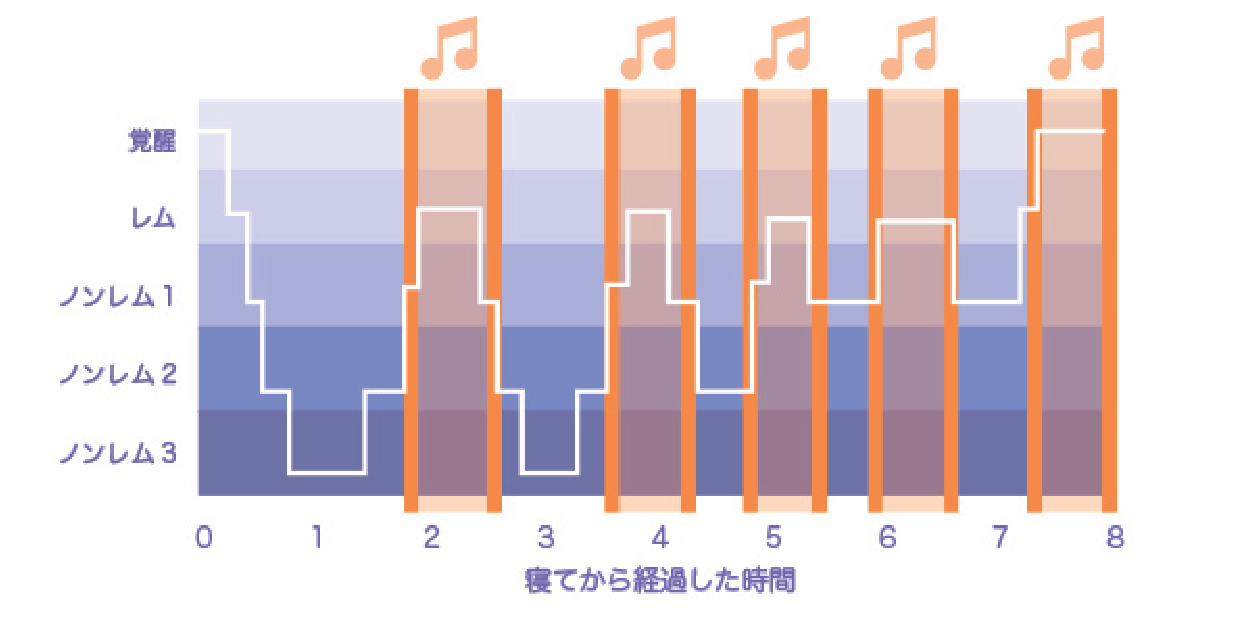
\includegraphics[width=15cm]{eps/remNonrem.eps}
\caption{音刺激提示のタイミング}
\label{melodyGraph}
\end{center}
\end{figure}


一晩中のx軸の数値、音楽の再生状況、夢日記の結果はデータベースをクラウドであるParseに保存する。図\ref{system}に一連のプログラムの流れを記載する。
\begin{figure}[htbp]
\begin{center}
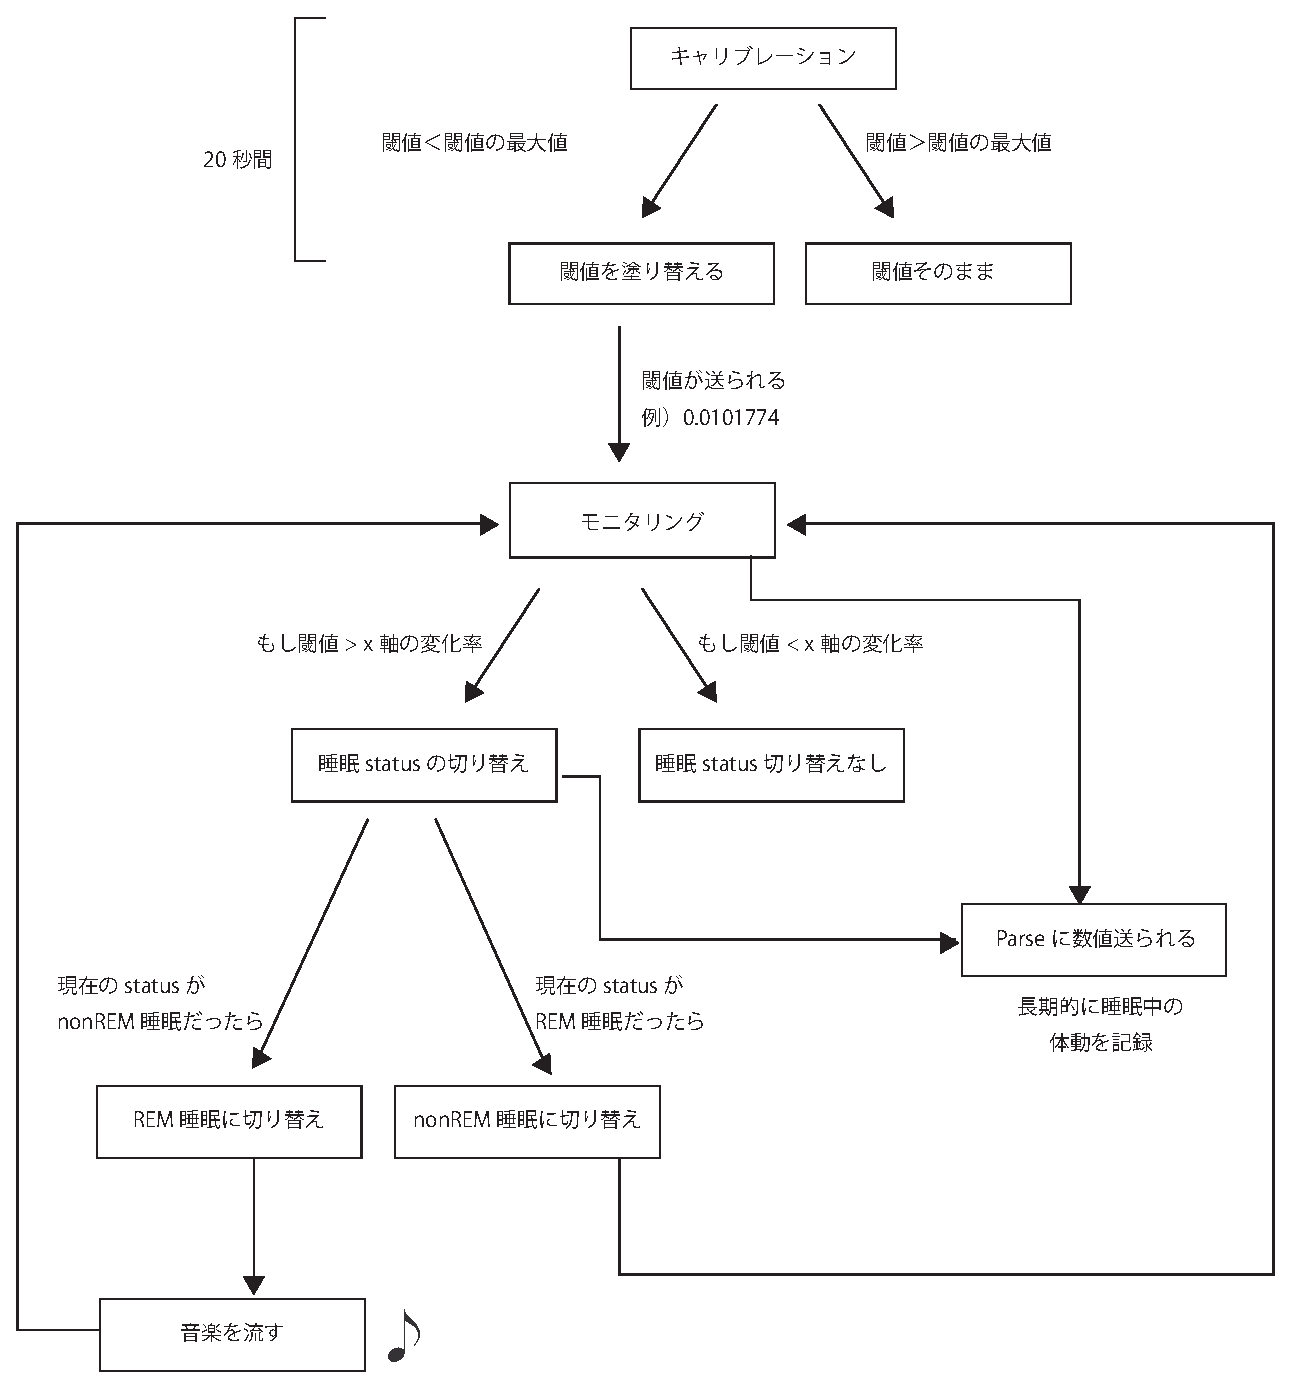
\includegraphics[width=15cm]{eps/system.eps}
\caption{DreamDateのフローチャート}
\label{system}
\end{center}
\end{figure}

\subsection{利用方法}
 ユーザーには予め記憶を思い起こさせる音と画像を登録してもらう。音選びは適している音声と適さない音声があるため注意する必要がある。使用してはいけない音は人の声だ。特に喋りかけてくるような内容の音声は、ユーザーを起こしてしまう可能性が高いということが実験結果から分かった。詳しくは第6章で述べる。逆に適している音は繰り返しある環境下で聞いていた音である。
 アプリの起動後、\ref{le01}のような画面が表示される。そこには「自動ロック機能をOFFにする」「音量は1〜3に設定する」やiPhoneの置く位置などの指示が書かれている。次に\ref{le02}の画面に遷移し、ユーザーの思い出に関連性のある画像を表示する。ここでは寝る前に記憶の情景を思い出す機会を与えている。そして\ref{le03}の画面では思い出の音楽が流れる。音楽を聴きながら、旅先での空間、香り、音の細部までを思い出して、気持ちを落ちつかせて瞑想状態に入ってもらう。次に\ref{le04}の画面に移動する。ユーザーは寝る前にアプリを起動してスタートボタンを押し、起動させたままスクリーンを伏せて枕の横に置く。20〜30分間後にDreamDateの加速度が起動をし一晩中ユーザーの体動のトレッキングが行われ、REM睡眠を検知すると音楽がなる。起床後\ref{le05}の画面で、ユーザーは起床すると夢の内容を忘れないように日記に投稿する。

\begin{figure}[htbp]
 \begin{minipage}{0.45\hsize}
  \begin{center}
   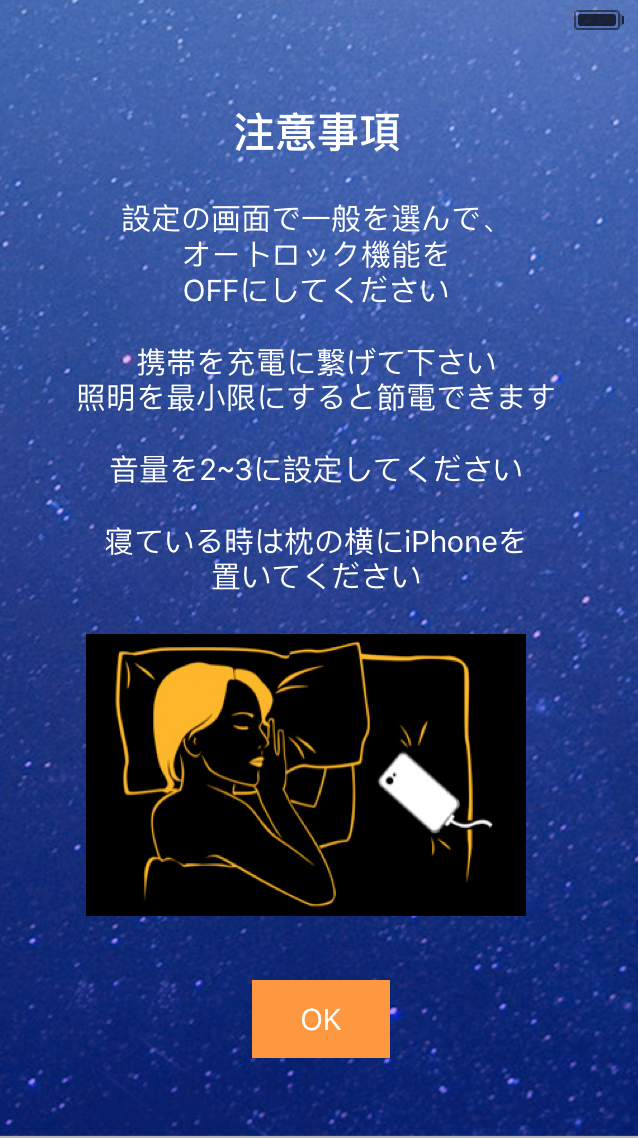
\includegraphics[height=90mm]{eps/AppIntro.eps}
  \end{center}
  \caption{起動画面}
  \label{le01}
 \end{minipage}
 \begin{minipage}{0.45\hsize}
  \begin{center}
   \includegraphics[height=90mm]{eps/AppMemoryImages.eps}
  \end{center}
  \caption{思い出の画像を表示}
  \label{le02}
 \end{minipage}
\end{figure}

\begin{figure}[htbp]
 \begin{minipage}{0.45\hsize}
  \begin{center}
   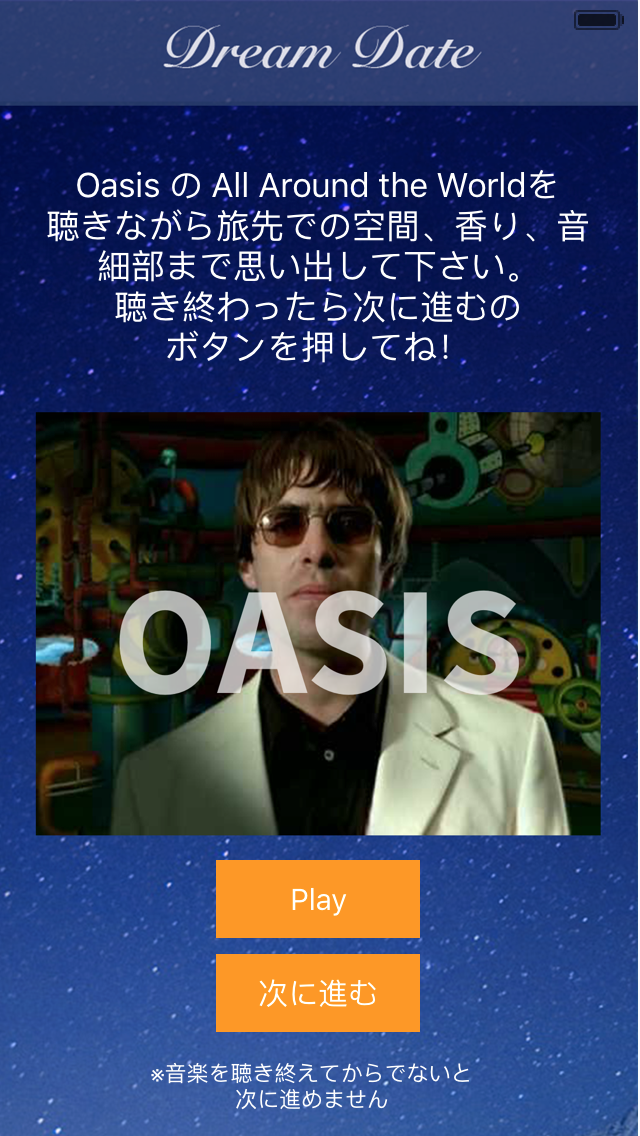
\includegraphics[height=90mm]{eps/AppMusicPlay.eps}
  \end{center}
  \caption{思い出に関連した音刺激の提示}
  \label{le03}
 \end{minipage}
 \begin{minipage}{0.45\hsize}
  \begin{center}
   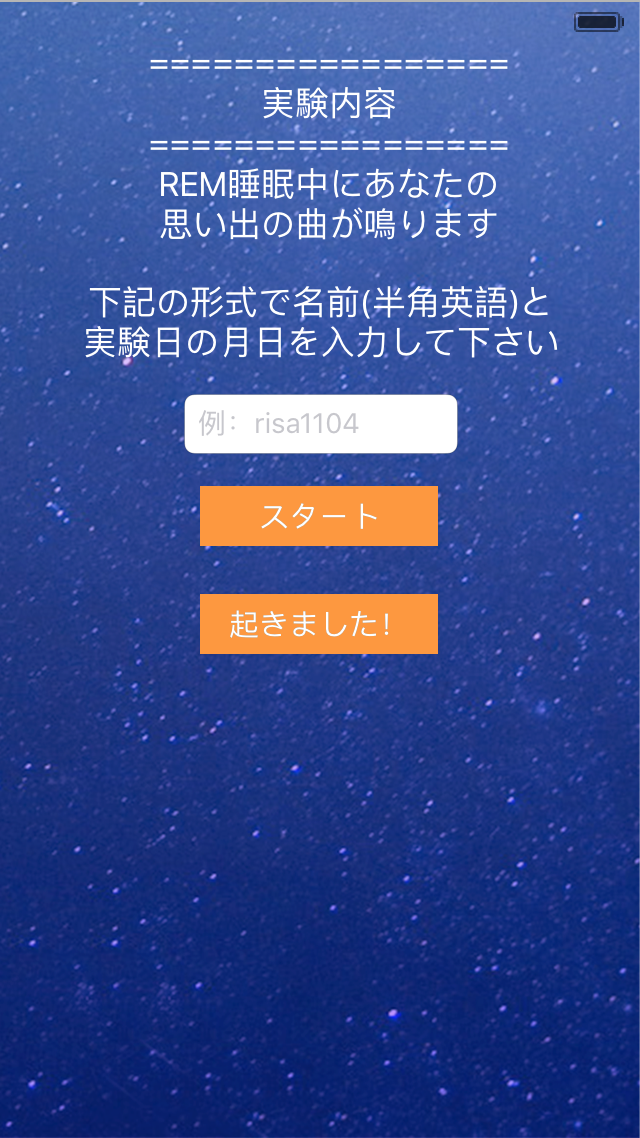
\includegraphics[height=90mm]{eps/AppStart.eps}
  \end{center}
  \caption{睡眠開始ボタン}
  \label{le04}
 \end{minipage}
\end{figure}

\begin{figure}[htbp]
 \begin{minipage}{0.45\hsize}
  \begin{center}
   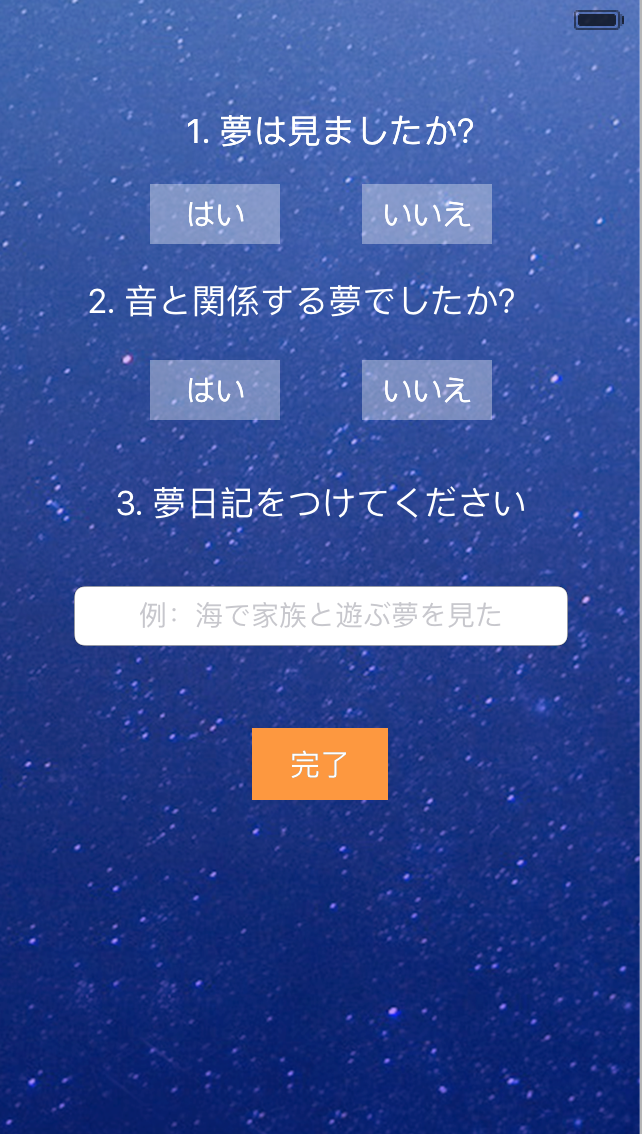
\includegraphics[height=90mm]{eps/AppDiary.eps}
  \end{center}
  \caption{夢日記記入ページ}
  \label{le05}
 \end{minipage}
 \begin{minipage}{0.45\hsize}
 \end{minipage}
\end{figure}
